\documentclass[serif,mathserif,final]{beamer}
\mode<presentation>{\usetheme{Calopsita}}
\usepackage{amsmath,amsfonts,amssymb,pxfonts,eulervm,xspace}
\usepackage{graphicx}
\usepackage[utf8]{inputenc}
\usepackage[brazil]{babel}
\graphicspath{{./figures/}}
\usepackage[orientation=landscape,size=a2,scale=0.8,debug]{beamerposter}

%-- Header and footer information ----------------------------------
% \newcommand{\footleft}{http://github.com/caelum/calopsita}
% \newcommand{\footright}{shawn at shawn lankton dot com}
\newcommand{\calopsita}{Calopsita}
\newcommand{\opensource}{\textit{open source}}

\title{Calopsita: um gerenciador de projetos ágeis}
\author{Alunos: Cauê Haucke Porta Guerra, Cecilia Fernandes, Lucas Cavalcanti dos Santos}
%-------------------------------------------------------------------


%-- Main Document --------------------------------------------------
\begin{document}
\begin{frame}{}
  \begin{columns}[t]

    %-- Column 1 ---------------------------------------------------
    \begin{column}{0.32\linewidth}

      %-- Block 1-1
      \begin{block}{Introdução}
        O \calopsita{} é um projeto que nasceu da necessidade de se trabalhar e gerenciar diferentes projetos ágeis, cada um com suas particularidades. Em especial, surgiu da necessidade de se trabalhar com equipes distribuídas em projetos ágeis. 
      \end{block}

      %-- Block 1-2
      \begin{block}{Funcionalidades}
        You can make a poster very quickly and easily by cutting and pasting
        the \LaTeX~codes from the paper!
      \end{block}

      %-- Block 1-3
      \begin{block}{BDD}
        The columns will automatically align with each other and try to look
        as nice as possible.  You may have to add {\tt$\backslash$vspace\{1pt\}}
        commands to adjust the spacing here and there.  Remember that you can
        use positive or negative numbers.
      \end{block}

    \end{column}%1

    %-- Column 2 ---------------------------------------------------
    \begin{column}{0.32\linewidth}

      %-- Block 2-1
      \begin{block}{Plugins}
        \begin{itemize}
          \item You can make
          \item lists, that
          \item allow people to see quickly
        \end{itemize}
      \end{block}

      %-- Block 2-2
      \begin{block}{Math}
        Include math within the text is as simple as $1+1=2$.  You can also
        highlight more important equations like this:
        \begin{equation*}
          \int_0^1\sin(x)+\cos^2(x)+\alpha x~d\!x
        \end{equation*}
      \end{block}

      %-- Block 2-3
			\begin{block}{Implementação}
				O \calopsita{} foi desenvolvido buscando o máximo de expressividade. Além disso, aproveitamos
				para testar novas tecnologias e padrões:
				
				\begin{itemize}
					\item{SeleniumDSL: DSL para manipulação do Selenium. Acresentamos suporte ao HtmlUnit, permitindo
					que nossos testes de integração fossem executados mais rapidamente;}
					\item{Vraptor3: como o \calopsita{} foi o primeiro projeto a utilizar o Vraptor3, ainda em suas
					versões betas, o uso que fazíamos dele fez com que vários pontos fossem alterados - melhorar}
					\item{ActiveRecord: adotamos como persistência no lugar de DataMapper}
					\item{REST: Aproveitando o suporte de VRaptor a REST}
				\end{itemize}
      \end{block}

    \end{column}%2

    %-- Column 3 ---------------------------------------------------
    \begin{column}{0.32\linewidth}

      %-- Block 3-1
      \begin{block}{Resultados}
        \begin{figure}[htb]
         \centering
				\fbox{
         	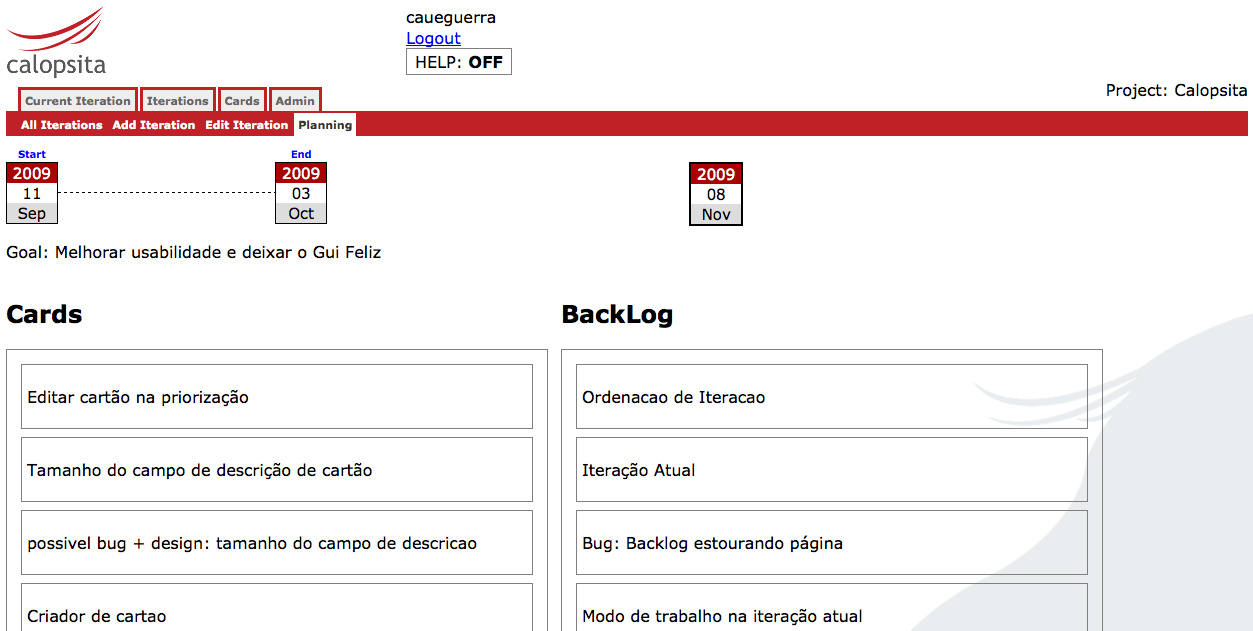
\includegraphics[width=.8\columnwidth]{images/planejamento}
				}
				\caption{Planejamento}
        \end{figure}
				
				\begin{figure}[htb]
         \centering
				\fbox{
         	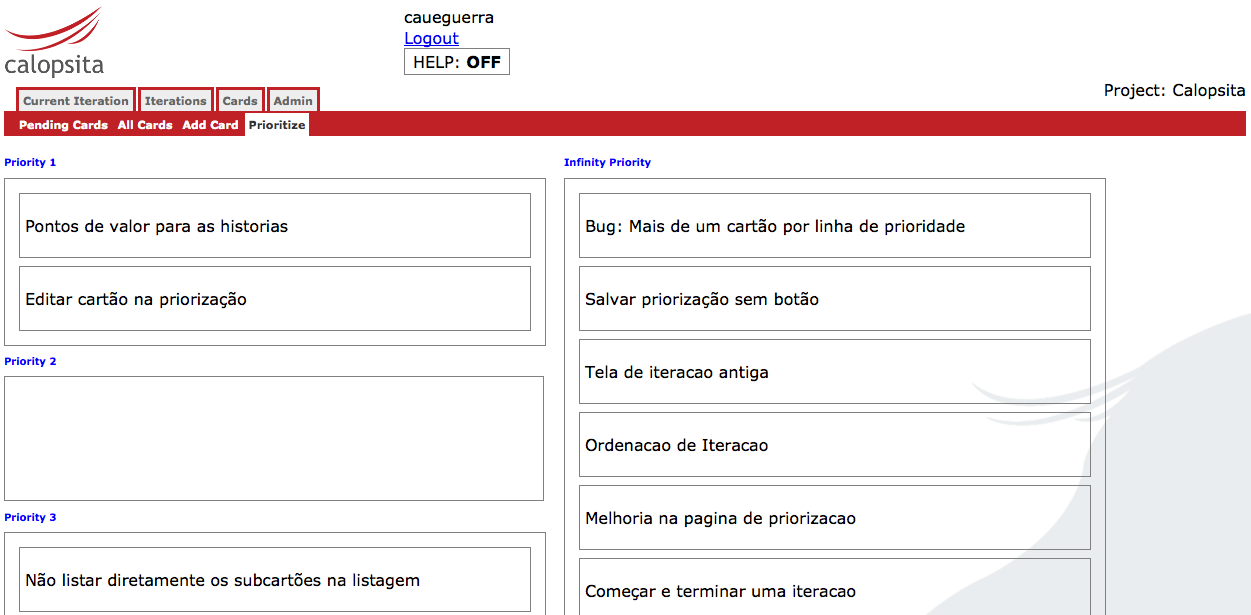
\includegraphics[width=.8\columnwidth]{images/priorizacao}
				}
				\caption{Priorização}
        \end{figure}

				\begin{figure}[htb]
         \centering
				\fbox{
         	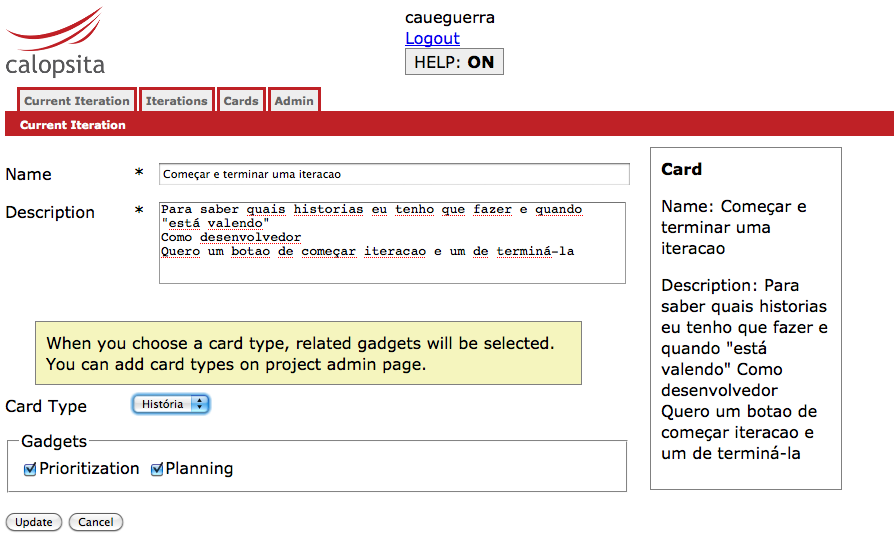
\includegraphics[width=.8\columnwidth]{images/cartao}
				}
				\caption{Cartões}
        \end{figure}
      \end{block}

    \end{column}%3

  \end{columns}
\end{frame}
\end{document}
